\chapter{Reprodução assexuada e clonagem nas plantas}\label{ch:b2:asexual-reproduction}

Num vale de Utah ergue-se uma floresta de quarenta e sete mil troncos
de álamo que é uma única planta: todos os troncos cresceram do mesmo
sistema de raízes, todas as células levam o mesmo genoma, e o
indivíduo tem cerca de catorze mil anos e pesa seis mil toneladas.
Todos os morangos de uma mesma variedade numa caixinha de supermercado
são pedaços de uma única planta multiplicada por estolões; todas as
bananas Cavendish da Terra são uma estaca de uma estaca de uma única
planta. As plantas, ao contrário da maioria dos animais, conseguem
produzir novos indivíduos sem sexo --- a partir de um caule, de uma
raiz, de uma folha, de uma única célula num frasco. Este capítulo
examina como elas fazem isso, como os agricultores o exploram e o que
custa a uma linhagem abrir mão da \omterm{def:b2:meiosis-heredity:meiosis}{meiose} e da fecundação: a questão de
por que o sexo existe.

\section{A multiplicação vegetativa}

\begin{definition}[Clone, geneta, rameta]\label{def:b2:asexual-reproduction:clone}
\index{clone}\index{geneta}\index{rameta}\index{multiplicação vegetativa}
A \emph{reprodução assexuada} produz novos indivíduos a partir de um
único genitor apenas por mitose, sem \omterm{def:b2:meiosis-heredity:meiosis}{meiose} nem fecundação: os
descendentes formam um \emph{clone}, geneticamente idêntico ao genitor
e entre si, exceto pelas \omterm{def:b2:genome-diversification:mutation}{mutações} somáticas que se acumulam. Nas
plantas, a forma habitual é a \emph{multiplicação vegetativa}, na qual
uma parte do corpo --- caule, raiz, folha --- enraíza e se torna uma
planta separada. Uma \emph{geneta} é o indivíduo genético, tudo o que
cresceu a partir de um zigoto; uma \emph{rameta} é uma unidade
fisiologicamente separada dela. Um canteiro de morangos pode conter mil
rametas de uma geneta; a floresta de álamos é uma geneta. A
multiplicação vegetativa é possível porque as células vegetais
conservam a capacidade de se dividir e de formar qualquer órgão --- são
\emph{totipotentes} --- e porque as plantas crescem a partir de
meristemas que podem ser reativados quase em qualquer lugar.
\end{definition}

\begin{proposition}[Os órgãos da multiplicação vegetativa]\label{prop:b2:asexual-reproduction:organs}
\index{estolão}\index{rizoma}\index{tubérculo}\index{bulbo}
As plantas desenvolveram o mesmo recurso a partir de todos os órgãos. A
partir do caule: os \emph{estolões} ou \emph{estolhos}, ramos
horizontais rente ao solo
que enraízam nos nós (morangueiro, ranúnculo-rasteiro); os
\emph{rizomas}, caules subterrâneos horizontais que se ramificam e se
fragmentam (grama-francesa, íris, gengibre, samambaia-das-taperas); os
\emph{tubérculos}, extremidades de rizoma intumescidas que armazenam
amido e levam gemas, os ``olhos'' (batata); os \emph{cormos}, bases de
caule verticais intumescidas (açafrão); os \emph{bulbilhos}, pequenos
bulbos formados nas axilas das folhas ou na inflorescência (alho,
algumas cebolas). A partir das folhas: os \emph{bulbos}, gemas envoltas
em folhas carnosas de reserva que se dividem em bulbos-filhos (cebola,
tulipa); plântulas ao longo da margem da folha, já com raízes, que se
desprendem (\emph{Kalanchoe}). A partir das raízes: os \emph{rebentos},
ramos que brotam de raízes horizontais (álamo, abrunheiro, framboeseira).
Por \emph{fragmentação}: um pedaço de ramo de salgueiro que flutua para
longe e enraíza, uma fronde de lentilha-d'água que se divide. Em todos
os casos, um órgão de reserva ou um meristema é levado a uma curta
distância, e a filha começa a vida com um suprimento de alimento que
nenhuma \omterm{def:b2:angiosperm-reproduction:seed}{semente} iguala.
\end{proposition}

\begin{omfigure}
\begin{tikzpicture}[every node/.style={font=\scriptsize}]
  % runner
  \begin{scope}
    \draw[thick] (0,0) -- (3.6,0);
    \foreach \x in {0,1.8} { \draw[thick, omExo!70!black, fill=omExo!30] (\x,0) .. controls (\x-0.3,0.6) and (\x+0.3,0.6) .. (\x,0); \foreach \a in {60,90,120} \draw[thick, omExo!70!black] (\x,0) -- ++(\a:0.7); \draw[gray] (\x,0) -- ++(-100:0.4) (\x,0) -- ++(-70:0.4); }
    \draw[thick, omThm] (0.2,0.15) .. controls (0.9,0.55) and (1.2,0.55) .. (1.8,0.1);
    \draw[thick, omThm] (2.0,0.15) .. controls (2.7,0.55) and (3.0,0.55) .. (3.5,0.1);
    \draw[thick, omExo!70!black] (3.5,0.1) -- ++(80:0.4); \draw[gray] (3.5,0.1) -- ++(-80:0.3);
    \node[below, align=center] at (1.8,-0.55) {estolão (morangueiro):\\um ramo horizontal enraíza nos nós};
  \end{scope}
  % rhizome and tuber
  \begin{scope}[xshift=5.2cm]
    \draw[gray, dashed] (-0.2,0) -- (3.8,0);
    \draw[very thick, omProp!80!black] (0,-0.5) -- (3.4,-0.5);
    \foreach \x in {0.6,2.0} \draw[thick, omExo!70!black] (\x,-0.5) -- (\x,0.7) (\x,0.3) -- ++(40:0.4) (\x,0.3) -- ++(140:0.4);
    \draw[thick, omProp!80!black, fill=omProp!40] (3.4,-0.5) ellipse (0.45 and 0.3);
    \foreach \p in {(3.2,-0.3),(3.6,-0.35),(3.7,-0.6)} \fill[omThm] \p circle (0.04);
    \foreach \x in {0.3,1.3,2.5} \draw[gray] (\x,-0.5) -- (\x,-0.9);
    \node[below, align=center] at (1.8,-1.05) {rizoma e tubérculo (batata):\\caules subterrâneos,\\gemas (olhos) no tubérculo};
  \end{scope}
  % bulb
  \begin{scope}[xshift=12.2cm]
    \draw[thick, fill=omExo!15] (0,-0.9) .. controls (-0.9,-0.6) and (-0.9,0.9) .. (0,1.0) .. controls (0.9,0.9) and (0.9,-0.6) .. (0,-0.9);
    \foreach \r in {0.55,0.35} \draw[thick] (0,-0.75) .. controls (-\r,-0.5) and (-\r,0.6) .. (0,0.8) .. controls (\r,0.6) and (\r,-0.5) .. (0,-0.75);
    \fill[omExo!60!black] (-0.1,-0.75) rectangle (0.1,0.3);
    \draw[thick, omThm, fill=omThm!30] (0.35,-0.5) ellipse (0.15 and 0.3);
    \foreach \x in {-0.3,0,0.3} \draw[gray] (\x,-0.9) -- (\x,-1.25);
    \node[below, align=center] at (0,-1.3) {bulbo (cebola):\\folhas carnosas,\\um bulbo-filho (vermelho)};
  \end{scope}
\end{tikzpicture}

{\small Três órgãos de \omterm{def:b2:asexual-reproduction:clone}{multiplicação vegetativa}: estolões que enraízam
nos nós, um caule subterrâneo que se intumesce num tubérculo e um bulbo
que forma um bulbo-filho. Em todos os casos, uma gema viaja com seu
alimento.}
\end{omfigure}

\begin{omfigure}
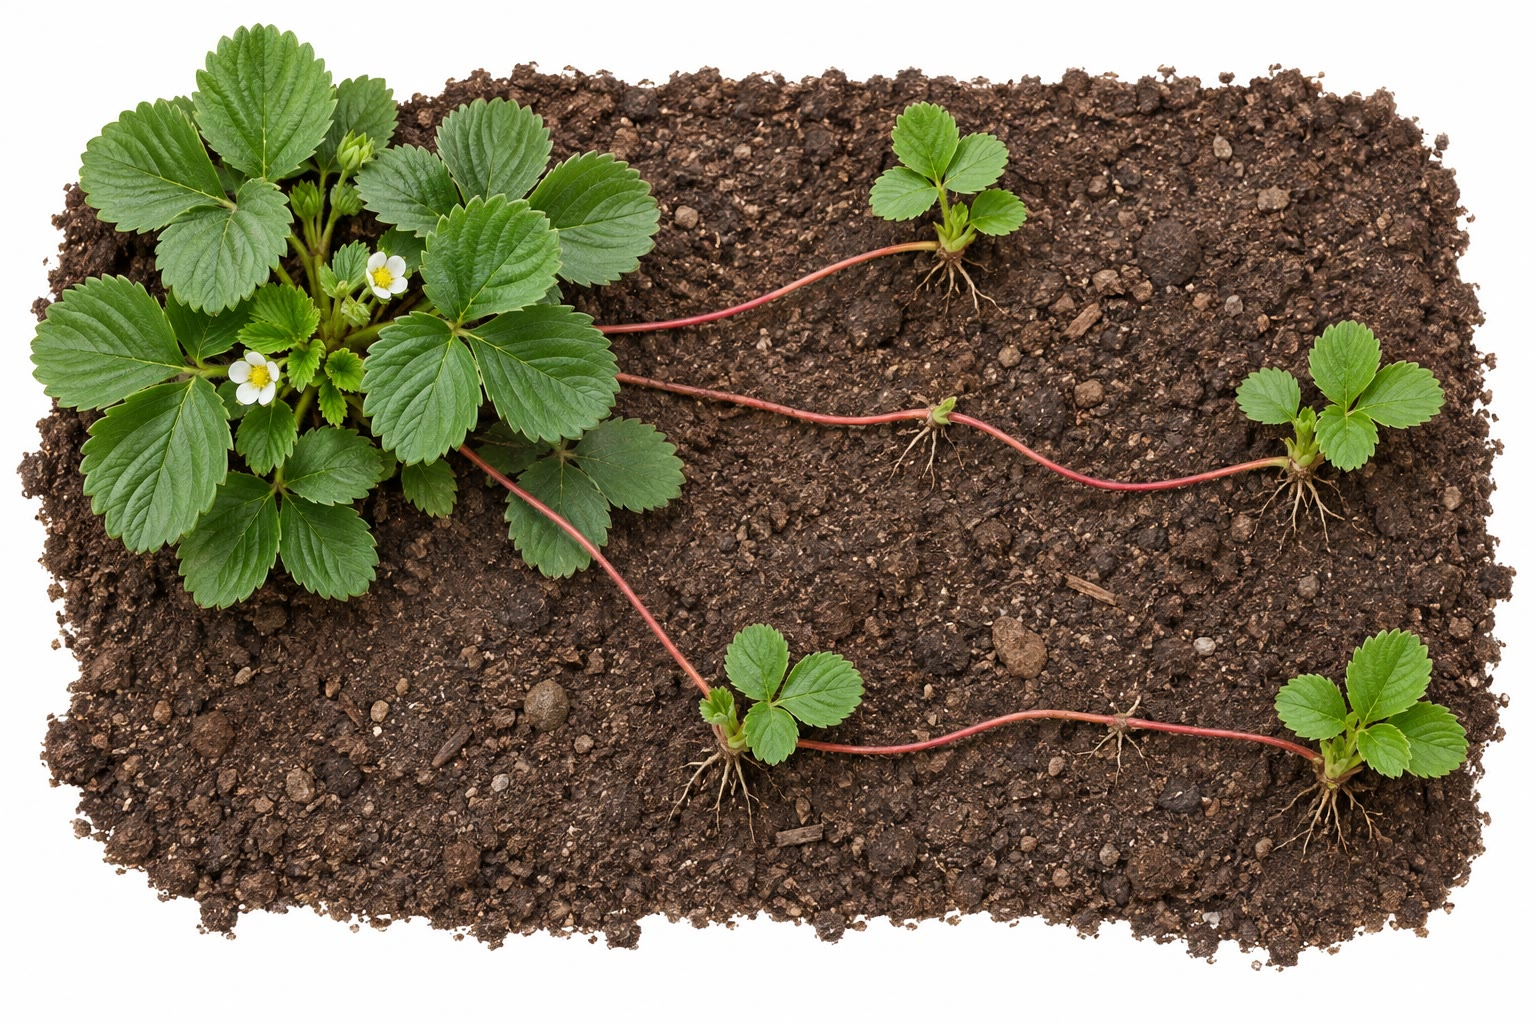
\includegraphics[width=0.46\linewidth]{images/book4/ai/b4-07-strawberry-runners.jpg}\hspace{0.03\linewidth}
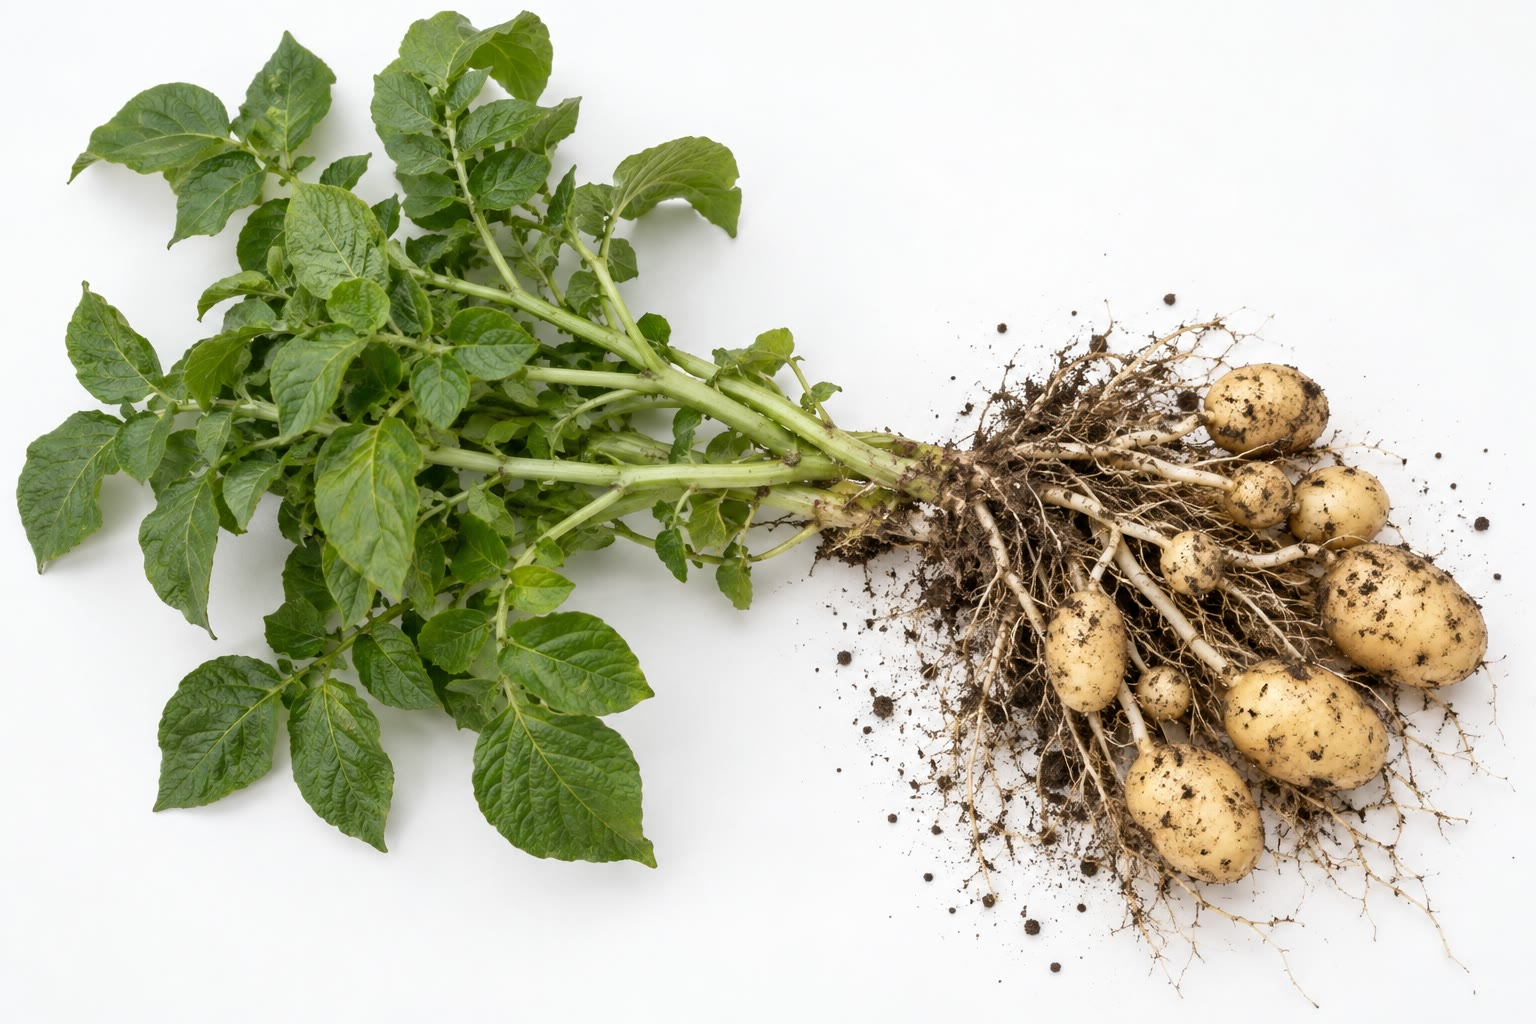
\includegraphics[width=0.46\linewidth]{images/book4/ai/b4-07-potato-tubers.jpg}

{\small À esquerda: um morangueiro e as plantas-filhas enraizando ao
longo de seus estolões. À direita: um pé de batata arrancado do solo,
com os tubérculos pendendo dos estolões --- cada tubérculo um pedaço de
caule que crescerá numa planta geneticamente idêntica a esta.}
\end{omfigure}

\begin{theorem}[A geometria de um clone que se expande]\label{thm:b2:asexual-reproduction:spread}
\index{crescimento clonal}
Uma \omterm{def:b2:asexual-reproduction:clone}{geneta} cujas \omterm{def:b2:asexual-reproduction:clone}{rametas} produzem cada uma $m$ filhas enraizadas por
ano, todas sobreviventes, cresce em número como
$N(t) = N_0 (1 + m)^t$ --- crescimento exponencial sem nenhum sexo ---
até que as \omterm{def:b2:asexual-reproduction:clone}{rametas} preencham o espaço em sua densidade de saturação
$d$ (\omterm{def:b2:asexual-reproduction:clone}{rametas} por unidade de área), após o que o \omterm{def:b2:asexual-reproduction:clone}{clone} avança como uma
frente. Um \omterm{def:b2:asexual-reproduction:clone}{clone} que estende seus estolões em linha reta à velocidade
$v$ tem, após $t$ anos, um raio $vt$, e o número de \omterm{def:b2:asexual-reproduction:clone}{rametas} cresce como
$\pi d (vt)^2$: de forma quadrática, e não exponencial. Um morangueiro
que lança estolões a \qty{0.5}{m} por ano tem um raio de \qty{5}{m}
após dez anos; o \omterm{def:b2:asexual-reproduction:clone}{clone} de álamos do parágrafo de abertura, de
\qty{43}{ha}, tem um raio de cerca de \qty{370}{m} e, com um avanço
líquido de alguns centímetros por ano, uma idade da ordem de $10^{4}$
anos --- coerente com a idade estimada a partir do recuo das geleiras.
\end{theorem}
\begin{proof}
Cada ano, cada \omterm{def:b2:asexual-reproduction:clone}{rameta} é substituída por ela mesma mais $m$ filhas, um
fator $1 + m$; $t$ anos dão $(1 + m)^t$. Uma vez preenchido o
interior, só as \omterm{def:b2:asexual-reproduction:clone}{rametas} da borda encontram espaço, e a borda avança à
velocidade dos estolões $v$; a área é $\pi(vt)^2$ e o número de \omterm{def:b2:asexual-reproduction:clone}{rametas}
é a área vezes a densidade.
\end{proof}

\begin{example}[Os organismos mais antigos]\label{ex:b2:asexual-reproduction:oldest}
O \omterm{def:b2:asexual-reproduction:clone}{clone} de álamos Pando (Utah) cobre \qty{43}{ha} com cerca de
\num{47000} troncos, cada um vivendo mais ou menos um século e sendo
substituído por rebentos das mesmas raízes; a \omterm{def:b2:asexual-reproduction:clone}{geneta} pode ter mais de
dez mil anos. Um \omterm{def:b2:asexual-reproduction:clone}{clone} da erva marinha \emph{Posidonia} no
Mediterrâneo se estende por \qty{15}{km} e pode ter cem mil anos; um
anel de arbusto-de-creosoto no deserto de Mojave foi datado em
\num{11700} anos, com os caules centrais morrendo à medida que o anel
se expande. Em todos os casos, o que é velho é a \omterm{def:b2:asexual-reproduction:clone}{geneta}; nenhuma célula
dela tem mais que algumas décadas, e o genoma foi copiado milhares de
vezes.
\end{example}

\section{Sementes sem sexo e animais sem pai}

\begin{definition}[Apomixia]\label{def:b2:asexual-reproduction:apomixis}
\index{apomixia}\index{partenogênese}
A \emph{apomixia} é a produção de \omterm{def:b2:angiosperm-reproduction:seed}{sementes} sem fecundação: um embrião
se desenvolve a partir de uma oosfera não reduzida (a célula-mãe do
\omterm{def:b2:plant-life-cycles:heterospory}{megásporo} pula a \omterm{def:b2:meiosis-heredity:meiosis}{meiose}) ou diretamente de uma célula do nucelo, e a
\omterm{def:b2:angiosperm-reproduction:seed}{semente} leva o \omterm{def:b2:meiosis-heredity:vocabulary}{genótipo} da mãe. O dente-de-leão, as hieracium, as
amoras-silvestres, a poa e muitos citros fazem isso; a \omterm{def:b2:angiosperm-reproduction:seed}{semente} dos
citros muitas vezes contém vários embriões, um sexuado e os demais
cópias nucelares da mãe. A apomixia conserva a \omterm{def:b2:angiosperm-reproduction:seed}{semente} --- sua
dispersão, sua \omterm{def:b2:angiosperm-reproduction:seed}{dormência}, seu envoltório --- e dispensa a \omterm{def:b2:meiosis-heredity:meiosis}{meiose}, de
modo que um \omterm{def:b2:meiosis-heredity:vocabulary}{genótipo} bem adaptado é difundido sem alteração; a maioria
dos apomíticos são \omterm{def:b2:genome-diversification:polyploidy}{poliploides} de origem híbrida, cuja \omterm{def:b2:meiosis-heredity:meiosis}{meiose} falharia
de qualquer forma. O equivalente animal é a \emph{partenogênese}, o
desenvolvimento a partir de um óvulo não fecundado: obrigatória em
alguns lagartos e nos rotíferos bdeloides, que não têm machos há
dezenas de milhões de anos; cíclica nos pulgões e nas pulgas-d'água,
que se multiplicam por partenogênese durante todo o verão, uma fêmea
dando à luz filhas vivas que já levam seus próprios embriões, e passam
no outono a uma geração sexuada que põe ovos de inverno.
\end{definition}

\begin{omfigure}
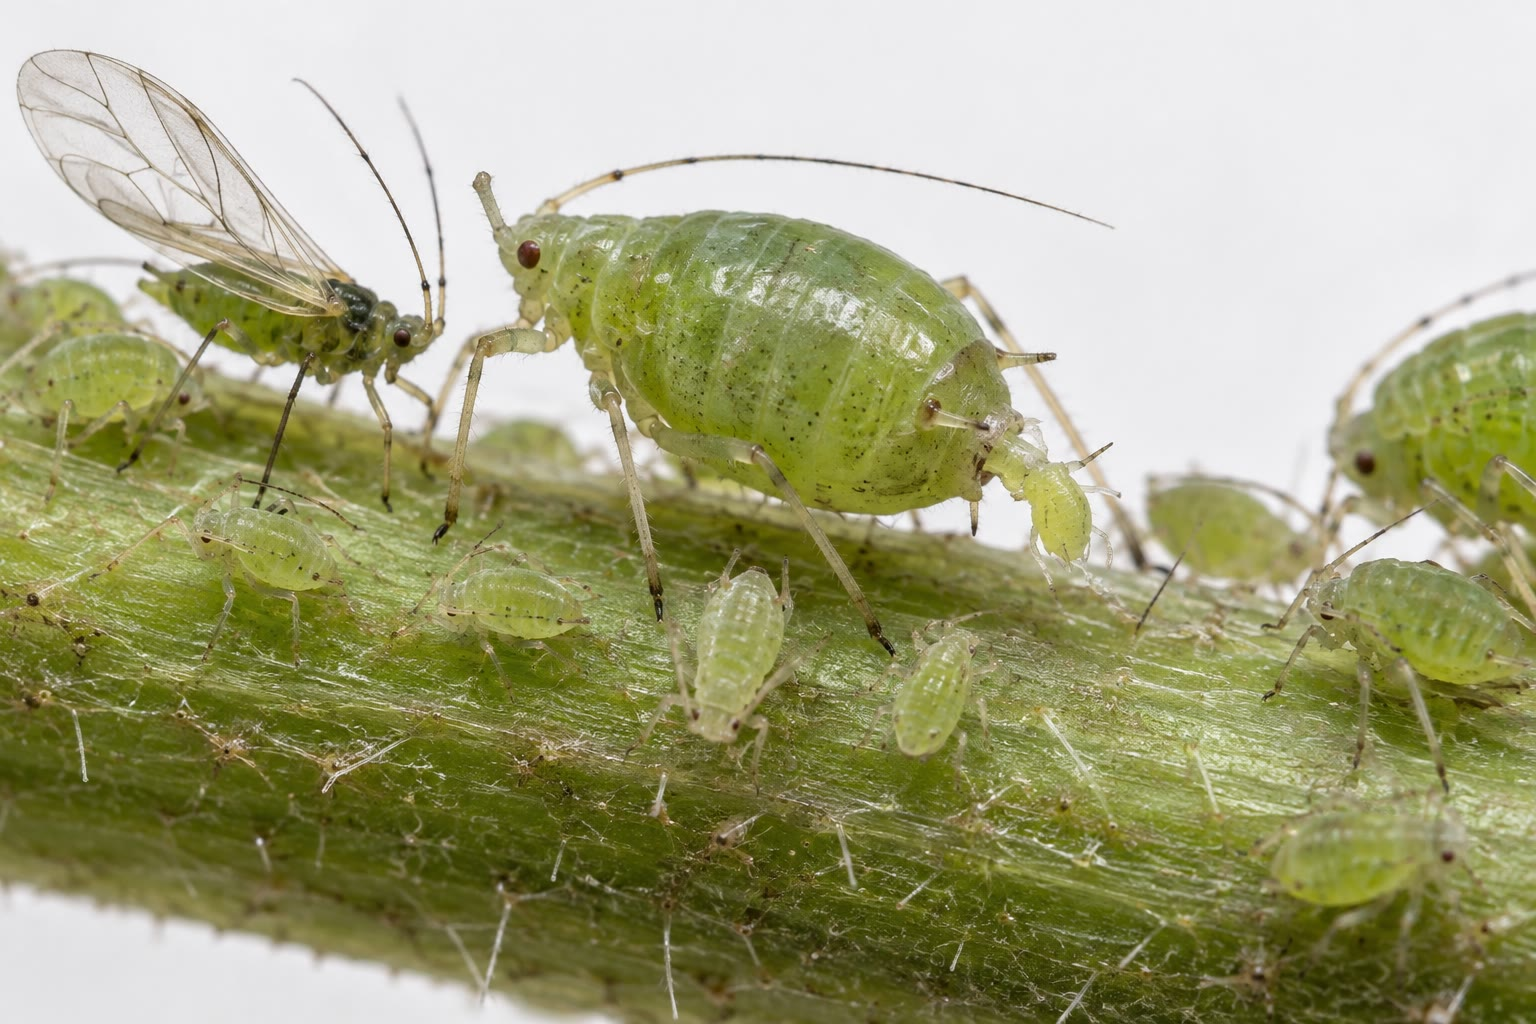
\includegraphics[width=0.55\linewidth]{images/book4/ai/b4-07-aphids.jpg}

{\small Pulgões sobre um caule: uma fêmea partenogenética áptera dando à
luz uma filha viva, ninfas de várias idades e uma migrante alada ---
um verão de crescimento exponencial sem um único macho.}
\end{omfigure}

\begin{example}[Um verão de pulgões]\label{ex:b2:asexual-reproduction:aphids}
Um pulgão partenogenético amadurece em cerca de oito dias e produz umas
cinco filhas por dia durante duas semanas; as filhas já nascem
grávidas (os embriões começam a se desenvolver dentro dos embriões da
mãe). Com um \omterm{def:b2:unicellular-diversity:division}{tempo de geração} perto de dez dias e uma taxa líquida de
aumento de cerca de \num{50} por geração, uma única fundadora em abril
poderia, sem freios, deixar $50^{12} \approx 2\times 10^{20}$
descendentes em outubro --- uma massa superior à da Terra. Joaninhas,
crisopídeos, vespas parasitoides, fungos e a chuva mantêm o número em
alguns milhares por planta, e a geração sexuada de outono reinicia o
\omterm{def:b2:asexual-reproduction:clone}{clone} em ovos recombinados antes do inverno.
\end{example}

\section{A clonagem pelo agricultor}

\begin{proposition}[Estaquia, mergulhia, enxertia]\label{prop:b2:asexual-reproduction:horticulture}
\index{estaca}\index{enxertia}\index{porta-enxerto}
Uma \emph{estaca} é um pedaço de caule, raiz ou folha induzido a
enraizar: a extremidade cortada forma um calo de células em divisão, do
qual surgem meristemas de raiz, com a ajuda da auxina (o hormônio de
enraizamento) e da umidade. A \emph{mergulhia} enraíza um ramo ainda
preso à planta e só depois o corta. A \emph{enxertia} une um ramo de
uma planta (o \emph{enxerto}) ao caule enraizado de outra (o
\emph{porta-enxerto}): os dois câmbios são pressionados um contra o
outro, um calo fecha o ferimento e novos xilema e floema se conectam
através dele em poucas semanas. A planta enxertada é uma quimera --- as
raízes conservam o genoma do porta-enxerto, o ramo que frutifica, o do
enxerto --- e o método só funciona entre plantas aparentadas (espécies
de um mesmo gênero, às vezes de uma mesma família), porque os tecidos
precisam reconhecer as células um do outro. Toda variedade de maçã,
pera, cereja, citros e uva é propagada por enxertia: uma variedade com
nome é uma \omterm{def:b2:asexual-reproduction:clone}{geneta}, mantida viva durante séculos por enxertos (as maçãs
Reinette datam do século XVI), e o porta-enxerto é escolhido segundo o
solo, a doença e o porte de árvore desejado --- os porta-enxertos
ananicantes produzem as árvores pequenas dos pomares modernos.
\end{proposition}

\begin{proposition}[Micropropagação e totipotência]\label{prop:b2:asexual-reproduction:tissueculture}
\index{micropropagação}\index{totipotência}\index{calo}
Qualquer célula vegetal viva com núcleo pode, em princípio, regenerar
uma planta inteira. Na \emph{cultura de tecidos}, um pedaço de tecido
esterilizado (um \emph{explante}: uma ponta de caule, um disco de
folha, uma antera) é colocado num meio de ágar com açúcar, minerais,
vitaminas e hormônios. Com auxina e citocinina em equilíbrio, as
células se desdiferenciam num \emph{calo}, uma massa de células não
especializadas em divisão; com mais citocinina que auxina, o calo forma
ramos; com mais auxina que citocinina, forma raízes; e, em algumas
espécies, forma \emph{embriões somáticos} --- embriões completos sem
oosfera. Os ramos são cortados e repicados a cada poucas semanas,
multiplicando-se por um fator de três a dez a cada vez, de modo que um
meristema dá um milhão de plântulas num ano. Como os vírus ficam
atrás da ponta em crescimento, um meristema caulinar com menos de um
milímetro costuma estar livre de vírus mesmo numa planta infectada: a
\emph{cultura de meristemas} é o modo como se limpam os estoques de
batata, morango, banana e orquídeas. O método é a prova prática da
totipotência, e a razão pela qual uma variedade vegetal pode ser
vendida aos milhões poucos anos depois de criada.
\end{proposition}
\begin{proof}[Evidências]
Skoog e Miller (1957) cultivaram calo de medula de tabaco em meios com
diferentes razões entre a auxina e a citocinina, recém-descoberta:
muita auxina dava raízes, muita citocinina dava ramos, um equilíbrio
dava apenas calo --- a formação dos órgãos era determinada por uma
razão entre dois hormônios, e não por uma substância formadora de
órgãos específica. Steward (1958) pôs em suspensão células isoladas e
pequenos grumos da raiz de uma cenoura num frasco giratório com água de
coco: alguns grumos formaram estruturas semelhantes a embriões que
cresceram em cenouras completas e floridas, o que mostrou que uma célula
diferenciada de um órgão maduro ainda contém, e pode usar, todo o
programa do desenvolvimento.
\end{proof}

\begin{omfigure}
\begin{tikzpicture}[every node/.style={font=\scriptsize}, >=stealth]
  \node[draw, rounded corners, fill=omDef!12, align=center] (ex) at (0,0) {explante\\(ponta de caule, disco de folha)};
  \node[draw, rounded corners, fill=omExo!30, align=center] (cal) at (4.6,0) {calo\\auxina $\approx$ citocinina};
  \node[draw, rounded corners, fill=omExo!30, align=center] (sh) at (8.4,1.2) {ramos\\citocinina $>$ auxina};
  \node[draw, rounded corners, fill=omExo!30, align=center] (rt) at (8.4,-1.2) {raízes\\auxina $>$ citocinina};
  \node[draw, rounded corners, fill=omDef!12, align=center] (pl) at (12.2,0) {plântulas\\aclimatadas no solo};
  \draw[->, thick] (ex) -- (cal) node[midway, below, align=center] {meio\\estéril};
  \draw[->, thick] (cal) -- (sh); \draw[->, thick] (cal) -- (rt);
  \draw[->, thick] (sh) -- (pl); \draw[->, thick] (rt) -- (pl);
  \draw[->, thick, omThm] (sh) .. controls (8.4,2.6) and (5.8,2.6) .. (5.2,0.6);
  \node[omThm, anchor=south] at (6.9,2.3) {repicagem a cada 4 semanas, $\times 5$};
\end{tikzpicture}

{\small Micropropagação: um explante é desdiferenciado num calo,
orientado para formar ramos ou raízes pela razão auxina/citocinina e
multiplicado por repicagens sucessivas antes que as plântulas sejam
aclimatadas ao solo.}
\end{omfigure}

\begin{omfigure}
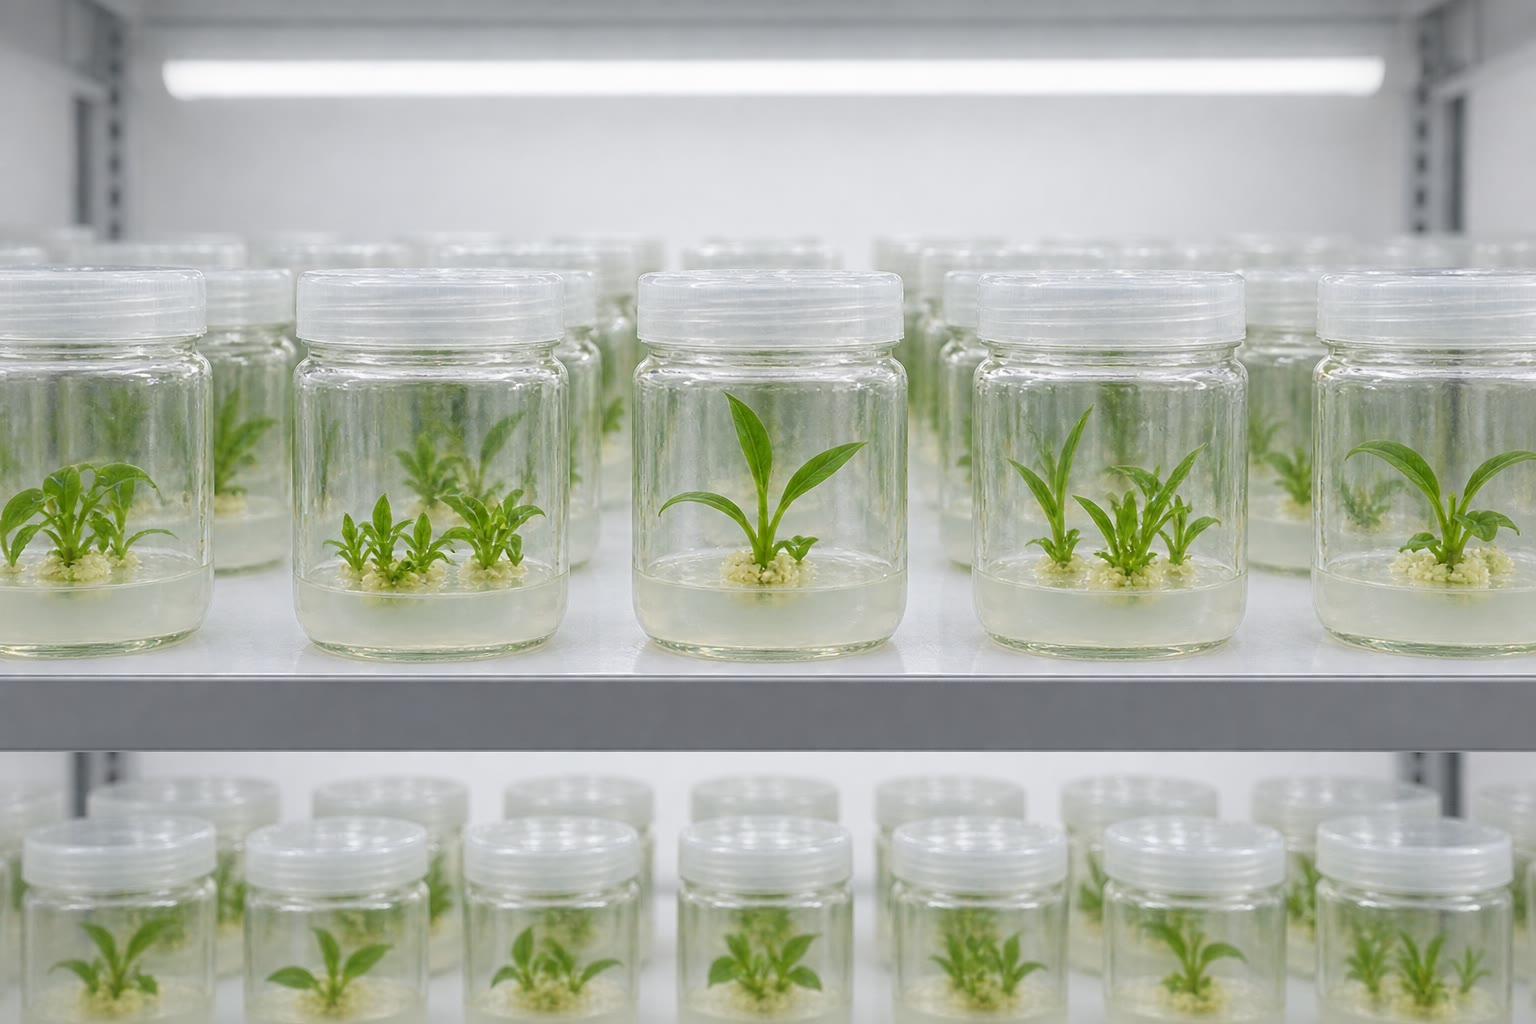
\includegraphics[width=0.6\linewidth]{images/book4/ai/b4-07-tissue-culture.jpg}

{\small Plântulas em ágar numa sala de crescimento: cada frasco contém
um \omterm{def:b2:asexual-reproduction:clone}{clone} da mesma variedade, multiplicado a partir de um único
meristema.}
\end{omfigure}

\section{O custo do sexo e o custo de dispensá-lo}

\begin{theorem}[O custo duplo do sexo]\label{thm:b2:asexual-reproduction:twofold}
\index{custo duplo do sexo}
Numa população em que cada fêmea produz $F$ descendentes, metade dos
quais machos, uma fêmea mutante assexuada que produz $F$ filhas, todas
cópias dela mesma, dobra sua parcela das fêmeas da geração seguinte.
Se a linhagem assexuada tem frequência $p$ entre as fêmeas, então, na
geração seguinte,
\[
p' = \frac{2p}{1 + p}, \qquad p_t = \frac{2^t p_0}{1 + (2^t - 1)p_0},
\]
de modo que, partindo de uma em mil, ela chega a metade da população em
dez gerações e à totalidade pouco depois. Tudo o mais sendo igual, o
sexo reduz à metade a taxa com que uma linhagem se multiplica --- o
preço de produzir machos. Como o sexo é, apesar disso, quase universal,
nem tudo o mais é igual: as linhagens sexuadas precisam ganhar, em
média, pelo menos um fator dois com a recombinação.
\end{theorem}
\begin{proof}
As fêmeas assexuadas são $pN$ e deixam $FpN$ filhas; as fêmeas
sexuadas são $(1 - p)N$ e deixam $F(1 - p)N/2$ filhas (a outra metade
são machos, que não produzem óvulos). A parcela assexuada das filhas é
$Fp/(Fp + F(1 - p)/2) = 2p/(1 + p)$. Escrevendo $q = p/(1 -
p)$, a recorrência se torna $q' = 2q$, de modo que $q_t = 2^t q_0$;
voltando à variável original, obtém-se $p_t$. Fazendo $p_t = \tfrac12$, obtém-se
$2^t q_0 = 1$, isto é,
$t = \log_2(1/q_0) \approx 10$ para $p_0 = 10^{-3}$.
\end{proof}

\begin{omfigure}
\begin{tikzpicture}
\begin{axis}[
  width=0.76\linewidth, height=5.6cm,
  axis x line=bottom, axis y line=left,
  xmin=0, xmax=20, ymin=0, ymax=1.05,
  xlabel={gerações}, ylabel={frequência da linhagem assexuada},
  xlabel style={font=\small, at={(axis description cs:0.5,-0.13)}, anchor=north},
  ylabel style={font=\small},
  tick label style={font=\small}, xtick={0,5,10,15,20}, ytick={0,0.5,1},
  legend style={font=\scriptsize, at={(0.5,-0.3)}, anchor=north, draw=none},
  clip=false,
]
\addplot[very thick, omThm, domain=0:20, samples=80] {2^x*0.001/(1+(2^x-1)*0.001)};
\addlegendentry{nenhuma outra diferença: domina em 12 gerações}
\addplot[very thick, omDef, domain=0:20, samples=80] {0.001*(1.3)^x/(1+(1.3^x-1)*0.001)};
\addlegendentry{os assexuados perdem \qty{35}{\%} da aptidão para parasitas: mais lento}
\addplot[very thick, omProp, domain=0:20, samples=80] {0.001*(0.9)^x/(1+(0.9^x-1)*0.001)};
\addlegendentry{os assexuados perdem \qty{55}{\%}: nunca se espalham}
\end{axis}
\end{tikzpicture}

{\small A vantagem dupla em ação. Partindo de uma em mil, uma linhagem
assexuada sem nenhuma outra desvantagem domina em uma dúzia de
gerações; só uma penalidade de aptidão de pelo menos metade --- por
parasitas, \omterm{def:b2:genome-diversification:mutation}{mutações} acumuladas ou adaptação mais lenta --- a contém.}
\end{omfigure}

\begin{proposition}[Para que serve o sexo]\label{prop:b2:asexual-reproduction:whysex}
\index{catraca de Muller}\index{hipótese da Rainha Vermelha}
Três benefícios são grandes o bastante para importar. A \emph{\omterm{prop:b2:asexual-reproduction:whysex}{catraca
de Muller}}: num \omterm{def:b2:asexual-reproduction:clone}{clone}, toda \omterm{def:b2:genome-diversification:mutation}{mutação} nociva é herdada por todos os
descendentes, e um genoma sem \omterm{def:b2:genome-diversification:mutation}{mutações}, uma vez perdido por acaso numa
população finita, nunca pode ser refeito; a carga sobe como uma
catraca, um dente de cada vez, e as pequenas populações assexuadas
degeneram. A recombinação reconstrói genomas limpos a partir de dois
genomas danificados. A \emph{adaptação}: duas \omterm{def:b2:genome-diversification:mutation}{mutações} úteis que surgem
em indivíduos diferentes de um \omterm{def:b2:asexual-reproduction:clone}{clone} competem e uma delas se perde;
numa população sexuada, elas se combinam (Fisher e Muller, década de
1930), de modo que as populações sexuadas se adaptam mais depressa
quando muitos genes precisam mudar. A \emph{Rainha Vermelha}: os
parasitas se adaptam ao \omterm{def:b2:meiosis-heredity:vocabulary}{genótipo} hospedeiro mais comum, e um \omterm{def:b2:asexual-reproduction:clone}{clone},
sendo um único \omterm{def:b2:meiosis-heredity:vocabulary}{genótipo}, é o mais comum de todos; os genitores
sexuados fazem de cada descendente uma fechadura nova. Caramujos,
peixes e plantas que têm populações sexuadas e clonais mostram as
sexuadas prevalecendo onde os parasitas são abundantes. As linhagens
assexuadas que prosperam --- dentes-de-leão, rotíferos bdeloides, a
maioria dos \omterm{def:b2:asexual-reproduction:clone}{clones} cultivados --- são jovens, ou são híbridos
\omterm{def:b2:genome-diversification:polyploidy}{poliploides} que carregam variação própria, ou são sustentadas por um
agricultor que mata os parasitas por elas.
\end{proposition}

\begin{example}[Monoculturas de um clone]\label{ex:b2:asexual-reproduction:monoculture}
Na década de 1840, a maior parte da batata cultivada na Irlanda era uma
única variedade clonal, a Lumper; o oomiceto \emph{Phytophthora
infestans}, chegando em 1845, encontrou um país de plantas
geneticamente idênticas, uniformemente suscetíveis, e destruiu a
colheita em três anos seguidos. A banana de exportação do mundo, até a
década de 1950, era um único \omterm{def:b2:asexual-reproduction:clone}{clone}, a Gros Michel, eliminada das
plantações da América Central por um fungo do solo; sua substituta, a
Cavendish, é igualmente um único \omterm{def:b2:asexual-reproduction:clone}{clone} e está sendo perdida, plantação
após plantação, para uma nova linhagem do mesmo fungo, contra a qual
não tem variação alguma a oferecer. Um \omterm{def:b2:asexual-reproduction:clone}{clone} é o alvo mais fácil da
natureza, e o agricultor que planta um precisa fornecer a resistência
que a recombinação teria fornecido de graça.
\end{example}

\section{Exercícios}

\begin{exercise}[$\star$]\label{exo:b2:asexual-reproduction:1}
Defina \omterm{def:b2:asexual-reproduction:clone}{clone}, \omterm{def:b2:asexual-reproduction:clone}{geneta} e \omterm{def:b2:asexual-reproduction:clone}{rameta}, e dê três órgãos naturais de
\omterm{def:b2:asexual-reproduction:clone}{multiplicação vegetativa}, com uma planta para cada um.
\end{exercise}

\begin{exercise}[$\star$]\label{exo:b2:asexual-reproduction:2}
Numa enxertia, que tecidos precisam se encontrar para que a união dê
certo, e com o que cada parceiro contribui para a árvore? Por que uma
árvore enxertada é uma quimera, e não um híbrido?
\end{exercise}

\begin{exercise}[$\star$]\label{exo:b2:asexual-reproduction:3}
Distinga a \omterm{def:b2:asexual-reproduction:apomixis}{apomixia} da \omterm{def:b2:asexual-reproduction:clone}{multiplicação vegetativa}, e a \omterm{def:b2:asexual-reproduction:apomixis}{partenogênese} de
ambas. Qual das três conserva a \omterm{def:b2:angiosperm-reproduction:seed}{semente}?
\end{exercise}

\begin{exercise}[$\star$]\label{exo:b2:asexual-reproduction:4}
Liste as etapas da micropropagação, do explante à planta no campo,
indicando as condições hormonais em cada uma.
\end{exercise}

\begin{exercise}[$\star\star$]\label{exo:b2:asexual-reproduction:5}
Um morangueiro produz 8 estolões por ano, cada um enraizando 3
plântulas, e cada plântula faz o mesmo no ano seguinte. Quantas plantas
haverá após 4 anos se nenhuma morrer? Com \qty{0.1}{m^2} por planta,
que área elas exigiriam? O que de fato limita o \omterm{def:b2:asexual-reproduction:clone}{clone}?
\end{exercise}

\begin{exercise}[$\star\star$]\label{exo:b2:asexual-reproduction:6}
O \omterm{def:b2:asexual-reproduction:clone}{clone} de álamos Pando tem \num{47000} troncos em \qty{43}{ha}, e
cada tronco vive cerca de \num{130} anos. Se a \omterm{def:b2:asexual-reproduction:clone}{geneta} tem \num{14000}
anos, quantas gerações de troncos ela já teve? Calcule seu avanço
radial médio em metros por ano, tratando-a como um disco.
\end{exercise}

\begin{exercise}[$\star\star$]\label{exo:b2:asexual-reproduction:7}
Um mutante assexuado surge com frequência $10^{-4}$ numa população
sexuada, com a mesma fecundidade. Calcule sua frequência após 5, 10 e
15 gerações. Quanto sua aptidão precisa ser reduzida para que ele nunca
se espalhe?
\end{exercise}

\begin{exercise}[$\star\star$]\label{exo:b2:asexual-reproduction:8}
Preveja o que faz um calo de tabaco em meios com razões auxina :
citocinina de 10 : 1, 1 : 1 e 1 : 10, e explique por que uma estaca de
caule é mergulhada em auxina, e não em citocinina.
\end{exercise}

\begin{exercise}[$\star\star$]\label{exo:b2:asexual-reproduction:9}
As batatas são plantadas como tubérculos. Um quilograma plantado rende
\qty{10}{kg}, e um hectare exige \qty{2}{t} de \omterm{def:b2:angiosperm-reproduction:seed}{batata-semente}.
Partindo de \qty{1}{kg} de uma nova variedade, quantas safras são
necessárias até que se possa plantar um hectare? Por que a \omterm{def:b2:angiosperm-reproduction:seed}{semente}
verdadeira permite uma multiplicação mais rápida, mas não é usada?
\end{exercise}

\begin{exercise}[$\star\star\star$]\label{exo:b2:asexual-reproduction:10}
Numa população clonal de $N$ indivíduos com $U$ \omterm{def:b2:genome-diversification:mutation}{mutações} nocivas por
genoma por geração, cada uma custando uma fração $s$ da aptidão, a
fração de indivíduos sem \omterm{def:b2:genome-diversification:mutation}{mutações} no equilíbrio é
$e^{-U/s}$ (deduzida no \cref{ch:b2:population-genetics}). Com $U =
0.1$ e $s = 0.02$, calcule o número de indivíduos sem \omterm{def:b2:genome-diversification:mutation}{mutações} para
$N = 10^{5}$ e $N = 10^{3}$, e explique, com a \omterm{prop:b2:asexual-reproduction:whysex}{catraca de Muller}, por
que a população pequena está condenada e a grande não --- ainda.
\end{exercise}

\begin{exercise}[$\star\star\star$]\label{exo:b2:asexual-reproduction:11}
Uma linhagem de patógeno capaz de vencer a resistência de um dado
\omterm{def:b2:meiosis-heredity:vocabulary}{genótipo} surge uma vez. Compare seu destino numa lavoura de um único
\omterm{def:b2:asexual-reproduction:clone}{clone} e numa população sexuada em que os genes de resistência segregam
em dez locos, cada um com dois \omterm{def:b2:meiosis-heredity:vocabulary}{alelos} de mesma frequência, e explique
nesses termos a grande fome irlandesa da batata.
\end{exercise}

\begin{exercise}[$\star\star\star$]\label{exo:b2:asexual-reproduction:12}
``O sexo custa um fator dois e está em toda parte; a assexualidade é
barata e rara.'' Discuta as três explicações do capítulo, e diga o que
os rotíferos bdeloides --- assexuados há quarenta milhões de anos ---
implicam para cada uma.
\end{exercise}

\section{Problema: Uma fazenda de morangos e um clone antigo}

\begin{problem}[{Problema de fim de semana --- a aritmética de um
clone, de uma lavoura de morangos preenchida por estolões e de um
laboratório que multiplica um meristema à invasão de uma população
sexuada por um apomítico e à degeneração genética de uma geneta
antiga, até o tempo para preencher a lavoura, as plântulas obtidas de
um meristema e o equilíbrio entre apomíticos e sexuados}]
\label{pb:b2:asexual-reproduction:1}
Um agricultor planta \num{100} morangueiros numa área de \qty{1}{ha}
que comporta \num{4} plantas por metro quadrado. Cada planta produz
\num{6} estolões por ano, cada um enraizando \num{2} filhas, e todas as
plantas sobrevivem. Um laboratório multiplica a mesma variedade por
cultura de tecidos: cada repicagem, a cada \num{4} semanas, multiplica
os ramos por \num{5}; \qty{80}{\%} das plântulas sobrevivem à
aclimatação. As estacas comuns da variedade estão \qty{90}{\%}
infectadas por vírus; as pontas de meristema de \qty{0.3}{mm} levam o
vírus com probabilidade $0.02$. Genoma do álamo: \qty{4.8e8}{} pares
de bases; \omterm{thm:b2:genome-diversification:rate}{taxa de mutação} somática de \qty{1e-9}{} por par de bases
por divisão celular; \num{20} divisões de células meristemáticas por
ano num ramo em crescimento.

\medskip
\noindent\textbf{Parte I --- Preencher a lavoura.}
\begin{enumerate}
  \item Quantas plantas a lavoura pode conter?
  \item Por que fator o número de plantas se multiplica a cada ano?
  \item Calcule o número de plantas após 1, 2 e 3 anos.
  \item Resolva $N(t) = 100\times 13^{t}$ para o instante em que a
        lavoura fica cheia.
  \item Uma vez cheia, só as plantas da borda de uma mancha encontram
        espaço. Se uma mancha avança \qty{0.5}{m} por ano, quantos anos
        uma planta levaria para cobrir a lavoura só pelo avanço?
  \item Explique por que o agricultor planta \num{100} plantas
        espalhadas pela lavoura, e não uma só.
\end{enumerate}

\medskip
\noindent\textbf{Parte II --- O laboratório.}
\begin{enumerate}[resume]
  \item Quantas repicagens são necessárias para passar de um meristema a
        pelo menos $10^{6}$ ramos? Quantas semanas?
  \item Quantas plantas sobrevivem à aclimatação?
  \item Qual é a probabilidade de que uma linhagem derivada de meristema
        esteja livre de vírus? E de que todas as \num{10} linhagens
        iniciadas a partir de uma planta estejam?
  \item O laboratório inicia \num{10} linhagens e descarta as
        infectadas após um teste. Número esperado de linhagens limpas?
        Compare com as estacas.
  \item Explique por que a ponta do meristema escapa do vírus.
  \item A lavoura poderia ser plantada com a produção do laboratório já
        no primeiro ano, em vez de preenchida por estolões em três.
        Dê uma vantagem e um risco de cada caminho.
\end{enumerate}

\medskip
\noindent\textbf{Parte III --- Um apomítico invade.}
Uma população de dentes-de-leão é sexuada; um mutante apomítico (que
clona as \omterm{def:b2:angiosperm-reproduction:seed}{sementes}) surge com frequência $p_0 = 10^{-3}$, com a mesma
produção de \omterm{def:b2:angiosperm-reproduction:seed}{sementes} por planta. Metade do esforço reprodutivo das
plantas sexuadas vai para o \omterm{def:b2:plant-life-cycles:heterospory}{pólen}.
\begin{enumerate}[resume]
  \item Justifique a recorrência $p' = 2p/(1 + p)$ para a frequência do
        apomítico entre os genitores de \omterm{def:b2:angiosperm-reproduction:seed}{sementes}.
  \item Calcule $p$ após 5 e 10 gerações, e a geração em que ele passa
        de metade.
  \item Um fungo causador de ferrugem se especializa no \omterm{def:b2:meiosis-heredity:vocabulary}{genótipo} mais
        comum: a produção de \omterm{def:b2:angiosperm-reproduction:seed}{sementes} do apomítico é reduzida por um
        fator $(1 - cp)$, com $c = 0.8$. Escreva a nova recorrência.
  \item Encontre a frequência de equilíbrio $p^*$ e verifique sua
        estabilidade pelo sinal de $p' - p$ de cada lado.
  \item Para que valores de $c$ o apomítico domina completamente?
  \item Calcule o equilíbrio para $c = 0.6$. Interprete: o que um
        parasita precisa fazer para proteger o sexo?
  \item O apomítico é triploide. Por que ele não pode voltar ao sexo, e
        por que isso importa a longo prazo?
\end{enumerate}

\medskip
\noindent\textbf{Parte IV --- O \omterm{def:b2:asexual-reproduction:clone}{clone} antigo.}
\begin{enumerate}[resume]
  \item Calcule o número de \omterm{def:b2:genome-diversification:mutation}{mutações} somáticas por divisão celular no
        álamo.
  \item Dois troncos do \omterm{def:b2:asexual-reproduction:clone}{clone} Pando estão separados por \num{14000}
        anos de crescimento de cada lado de seu ancestral comum. Quantas
        divisões celulares os separam, e quantas \omterm{def:b2:genome-diversification:mutation}{mutações} distinguem
        seus genomas?
  \item Que fração do genoma isso representa? Se \qty{2}{\%} do
        genoma for codificante, quantas diferenças codificantes?
  \item Um \omterm{def:b2:asexual-reproduction:clone}{clone} não tem \omterm{def:b2:meiosis-heredity:meiosis}{meiose} nem seleção no nível do organismo para
        eliminar essas \omterm{def:b2:genome-diversification:mutation}{mutações}. O que as elimina, e por que essa
        peneira é mais fraca que numa linhagem sexuada?
  \item Pando é ``geneticamente uniforme''? Discuta em duas frases.
  \item Enuncie o resultado: o tempo para preencher a lavoura por
        estolões, as plântulas que um meristema dá em um ano e a
        frequência de equilíbrio do apomítico para $c = 0.8$.
\end{enumerate}
\end{problem}
